\documentclass{article}[12pt]
\usepackage{graphicx}
\usepackage{tabularx}
\usepackage{natbib}

\usepackage{array}
\usepackage{amsmath}
%\usepackage[backend=bibtex]{biblatex}
\bibliographystyle{..//refs/styles/ecoletters.bst}
\setkeys{Gin}{width=0.8\textwidth}
%\setlength{\captionmargin}{30pt}
\setlength{\abovecaptionskip}{10pt}
\setlength{\belowcaptionskip}{10pt}
 \topmargin -1.5cm 
 \oddsidemargin -0.04cm 
 \evensidemargin -0.04cm 
 \textwidth 16.59cm
 \textheight 21.94cm 
 \parskip 7.2pt 
\renewcommand{\baselinestretch}{2}
\AtBeginEnvironment{thebibliography}{\linespread{1}\selectfont}
\parindent 0pt
\usepackage{lineno}
\linenumbers % for dissertation

%\usepackage{xr-hyper}
%\usepackage{hyperref}


\title{Phenological differences among species explain why early leafout extends the calendar but not thermal growing season}
%dl2024Sept20: I like the idea here, but struggle with the wording---"extends the calendar"--- it might be confusing to a reader unfamiliar with the concept

\author{Dan, Cat, Deidre and Lizzie}

\usepackage{Sweave}
\begin{document}
\Sconcordance{concordance:phen_framing.tex:phen_framing.Rnw:1 35 1 1 0 18 1 1 112 181 %
1}


\maketitle
%\setlength{\parskip}{0.5pt} % 1ex plus 0.5ex minus 0.2ex}
\setlength{\parindent}{0pt}

%cjc2024Sept25: I think Lizzie and Deirdre already hit the highlights for the Intro for now. I agree that there are paragraphs that need to be moved to the Results and Discussion (anything that includes the figures). I also think you need to set up the experiement a bit better in why it's so cool. A little more development on the latitudinal gradient would be good, even if the results aren't exciting, it'd be great to set up our initial hypothesis more. And maybe get into trees vs shrubs and interannual variation. This was a massive endeavor, I want the reader to be excited about it. 

\section{Introduction}
Carbon uptake by terrestrial plants is a major determinant of Earth's climate system \citep{} (say more precisely). In mid and high latitudes, net carbon uptake is primarily determined by the length of the growing season \citep{White1999}. Most models of carbon storage assume that earlier spring leafout with climate change will drive longer seasons and increased carbon storage, in part offsetting future warming \citep{Churkina2005,White1999,Keenan2014}. Recent findings, however, have called this critical assumption into question. 

%emwNov4 -- I would love to get Cat's help on citations in this paragraph (and throughout). I have offered some, but her ideas would be better.
Recent research has suggested that plants adjust their end of season timing dynamically such that longer seasons do not increase total productivity, but the mechanism---and prevalence---of this effect is unclear \citep{Zani2020,Norby2021,Zohner2023}. Observations have found that calendar growing seasons have lengthened with climate change \citep{Menzel1999,Liu2010}, but other studies have found that earlier leafout is often correlated with earlier end-of-season events \citep{Zani2020,Liu2016,Keenan2015}. Recent work has suggested early, increased productivity in the growing seasons drives early senescence \citep{Zani2020}, and proposed include that plants adjust mid-season based on a combination of growing season heat and daylength \citep{Zohner2023}. Such studies, however, are based generally on large-scale satellite measurements and small-scale single species pot experiments, and contrast with findings from long-term large-scale $CO_2$ enrichment studies (cite Norby2021). 



% Norby2021: 10.1126/science.abg1438

%emwNov4 -- This opening used to be more about carbon but I think, given our data, we may want to veer away from C and NPP a bit and just come back to it later.
These contrasting results suggest fundamental gaps in our understanding of how early-season events (and thermal conditions of the vegetative period?) shape growing season length. How early-season events, such as leafout, affect end-of-season events is poorly understood. While results from satellites (e.g., using NDVI) show a correlation,  what exactly is being measured for `end of season' is not clearly tied to a plant-scale event. Yet any connections would likely start at the individual plant level, where we rarely if ever have good measures of start and end of season events together. Further, because end-of-season events, are often more locally adapted---with plants using unique photoperiods to cue important events such as budset (CITES)---than start-of-season events, these trends may importantly vary across populations. Such population-level studies, however, are based on a very limited number of species \citep{Zeng2024}. Species generally vary strongly in their start-of-season phenology, with this being a major factor that can influence forecasts \citep{Morales-Castilla2024} and land surface models (CITES). Results to date reporting correlation between start- and end-of-season events generally cannot differentiate between different species, populations or individuals, making our inference limited. 
% Theory suggesting this is driven by different plant strategies in response to abiotic and biotic environmental pressures (CITES), and also predicts that they should vary strongly in end-of-season events ...

%emwNov8 -- I don't love the focus on variation ... we do get into species level variation but am not sure we want to ask this as the major question so I rewrote it, but left old text for now. 
Here, we examine how start-of-season events, using leafout, may affect end-of-season, using budset, to determine the length of the growing season.
% In this study, we test how variation in start-of-season---leafout--and end-of-season---budset---phenology among species, populations, and individuals affect the length of the growing season. 
We address this using rarely available plant-scale data---phenological observations over three years from a multi-species common garden study that can test how correlated leafout and budset are in different species across populations and examine which phenological event more strongly influences variation in growing season length. From this, we can understand how start- and end-of-season events together impact the calendar growing season, and its thermal conditions, which connect to potential productivity. This study offers insights into physiology that will allow us to scale from ecosystem level observations to individual mechanisms too, and improve forecasting. %emw2024Sep19 -- woo, woo

\section{Results \& Discussion} 
%emwNov8: Could finalize text a bit more but must-do before submitting to make sure all the numbers are correct in Rnw.


%emw2024Sep19 -- I liked your questions, I might group answering them in the results (and since people are confused about variance -- keep all that in ONE paragraph and simplify and clarify the answers to your questions ... this would be way easier with a combined results and discussion). 
%dl2024Sept20 I agree, if our question is which phase has the stronger influence then discussing them together might help make this comparison

We found an apparently fundamental---and unexpected trade-off---between early, longer growing seasons and the thermal growing season. In our common garden, earlier leafout led to earlier budset (Pearsons correlation coefficient of 0.32 $CI_{95}$[0.25, 0.39]) with  implications for the total length of the growing season. Measured in calendar days, the growing season remained consistent over the three year study period (Figure \ref{fig:vapar}c), despite substantial difference among years for leafout and budset. However, we found that a generally later leafout resulted in a longer thermal, or meteorological, growing season, defined here as the period of favorable meteorological conditions for plant growth \citep{Korner2023} (Figure \ref{fig:thermcal}c). 

These contrasting results---of a relatively stable growing season measured in calendar days, but one that is `shorter' in thermal time with earlier leafout---may explain some of the contrasting results of how climate change affects end-of-season events and productivity \citep{Zani2020}. Our results show that earlier leafout may have little effect on the thermal growing season because of unfavorably low temperatures combined with the observed correlation between leafout and budset (Fig XXa). Given that photosynthesis is temperature limited, earlier springs appear to provide limited opportunity for substantial growth yet may deprive plants of fully using late-season warmth. This may explain why multiple studies have failed to find correlations between longer seasons and increased plant growth (grephoneCITES). 
%The thermal growth season is likely a better proxy for carbon gain. Even with very weak carry-over effects between SoS and EoS, phenological advances that drive SoS into less favorable conditions for carbon assimilation in the early spring, trade more carbon gain in mid season for reduced gain in early. 
% The dynamics may help to explain why phenology advances with climate change have not clearly translated into higher levels of primary productive \citep{}. 

This relationship was strongly species-dependent. with later leafout leading to longer thermal seasons most apparent in species that typically leaf out earlier in the spring relative to others. This included shrubs such as \emph{Sambucus racemosa}, \emph{Viburnum cassiodes}, \emph{Spirea alba}, \emph{Diervella lonicera}, \emph{Aronia melanocarpa} \emph{Spirea tomentosa} and the tree species \emph{Betula populifolia}. Later-leafout species showed a weaker relationshio )(\emph{Betula papyrifera}, \emph{Betula allegheniensis} and \emph{Alnus incana}, Figure \ref{fig:thermcal}d). 
%cjc2024Sept25: I feel curious about upper temperature thresholds and what may be considered "too hot" for some species' productivity. Based on anecdotal evidence from Tree Spotters and these common garden observations, I remember some individuals dropping leaves in late summer before bud set because of drought-like conditions. I don't know if we can always assume that higher temperatures necessarily correlate to higher productivity - I'm thinking about assimilation curves and how they hit a peak at certain temperatures but begin to drop again with higher temps. 

We can see these dynamics play out by tracking the phenology of four individuals plants and an example. The earlier individual of \emph{Aronia melanocarpa} depicted in Figure \ref{fig:concept}a, starts growing 24 days before a later individual, but only ceases 13 days before it (i.e., it has a 14 day longer calendar growing season). However, because the 24 day growth advantage it has occurs when thermal conditions are less favorable, it ends up having a shorter thermal growing season (i.e., less change for carbon assimilation) than its later conspecific (Figure \ref{fig:concept}b). This is not the case for the later leafing species \emph{Myrica gale} where the both the earlier and later leafing individual start growing under more optimal thermal conditions, so the 20 day ``head start" the earlier individual incurs results in a both a longer calendar and thermal growing season (Figure \ref{fig:concept}a,c). 

\emph{Variation in leafout and budset}\\

Our common garden captured high variation in both leafout and budset, allowing us to examine how the two correlate, but also providing important insights into how both vary across species, populations and years. Consistent with a high number of studies finding species and year-to-year environmental variation drive leafout variation (CITES), we found high variance in leafout timing among species and years ($\sigma_{species}$: 8.23 $UI_{95}$[5.22,12.81], $\sigma_{year}$:10.49 $UI_{95}$[4.27,24.60], Figure \ref{fig:vapar}a,b). Population level variation was low ($\sigma_{population}$:0.62, $UI_{95}$[0.02,2.82], Figure \ref{fig:vapar}c). \emph{Sambucus racemosa} was typically the first species to leafout in the spring, leafing out approximately two weeks before \emph{Sorbus americana} the last species to leaf out (Figure \ref{fig:vapar}c). There were no differences in leafout timing among the four populations included in our study (Figure \ref{fig:vapar}c). Leafout was the earliest in 2019 and the latest in 2020 (Figure \ref{fig:vapar}c). %emwNov8: Add something to this paragraph that basically says: this jives with the whole climate change literature documenting big differences in spring and also with meta-analyses of common garden studies (Aitken and Bemmels, me and Zeng) that find leafout is not structured by population. 

Spring phenological phases are reported to be more plastic than autumn ones (CITES), but we found that, relative to leafout, variance in budset timing was higher for species, years and populations ($\sigma_{species}$: 9.81 $UI_{95}$[ 6.61,14.49], $\sigma_{year}$: 14.92 $UI_{95}$[5.68,9.21], $\sigma_{population}$: 2.35, $UI_{95}$[0.23,8.51], Figure \ref{fig:vapar}), but followed similar relative contributions (highest variance in year, lowest in population). Budset was earliest for \emph{Amelanchier canadensis} and latest for \emph{Alnus incana} and \emph{Betula paperifera} with more than three weeks between them (Figure \ref{fig:vapar}a). Following trends leafout and our finding that earlier leafout correlates with earlier budset, 2019 had the earliest budset and 2020 the latest (Figure \ref{fig:vapar}b).

%emwNov8: Can we put this 3 day number (below paragraph) in context compared to year to year variation? Also, why the grant? Also, we need to test FFD. 
These results are somewhat surprising as budset is commonly thought to be strongly dependent on population, with different populations requiring different critical photoperiods to trigger budset and leading to relatively stable budset dates across years (Soolanayakanahally2013, and find some review paper). Supporting this---and in contrast to leafout---we found that populations did vary in their budset. Populations from the Second College Grant set buds approximately three days before those from the white mountains, but these differences statistically weak (Figure \ref{fig:vapar}b) and small. Our results suggest we need much more work on additional species, as results to date have focused mainly on one species (\emph{Populus balsamifera}) and more efforts to understand how environmental factors beyond photoperiod may affect budset. Even for \emph{Populus balsamifera}, the species suggested to be mainly photoperiod-controlled, recent work suggests temperature may also play a major role (Michelson2018).   

% OLD text: The phenological carry-over effects between leafout and budset that we observed was interesting in light of the fact that spring phenological phases are reported to be more plastic than autumn ones (is this still true?). Some of this might have to do with scale of measurement---macro-scale measurements like remote sensing may detect different things. Budset is the end of primary growth which we observed closely  .... The low levels of phenological variance between populations in our common garden provide little evidence for local adaptation in phenology. We found slightly stronger evidence for budset than leafout, which is consistent with the literature \citep{}. 

%emwNov8: I did not update this paragraph much. 
High variation across species in both their leafout and budset timing lead to species to drive most variation in  growing season length  ($\sigma_{species}$: 14.38, $UI_{95}$[9.85,20.81], with less variation among years ($\sigma_{year}$: 4.67 $UI_{95}$[0.76,8.63], Figure \ref{fig:vapar}b) and little variation explained by population ($\sigma_{population}$: 2.50, $UI_{95}$[0.19,2.82], Figure \ref{fig:vapar}c). Due to it's early leafout and late budset \emph{S.racemosa} had the longest calendar growing season of the species in our study. \emph{A. canadensis} and \emph{S. americana} had the shortest growing seasons, though for \emph{A. canadensis} this was due to early budset and for \emph{S. americana} late leafout (Figure \ref{fig:vapar}a). Population level differences in calendar growing season were determined by differences in budset, and followed the same pattern with Grant marginally earliest and white mountains  latest, with high uncertainty. (Figure \ref{fig:vapar}b). 


\emph{Ecological and forecasting implications}\\
%emwNov8: I have not read the full R&D together... I suspect once you do, you can cut some of the below which might now be repetitive. 
Our multi-species common garden study showed that for already early leafing species, earlier leafout does not extend their thermal growing season---a proxy for potential carbon uptake period---despite extending the calendar growing season. For early leafout species, delayed leafout resulted in a longer thermal growing season. This relationship was in part explained by positive correlations between leafout and budset where later leafing individuals also set buds later, extending their growth into that later part of the season when thermal conditions were more favorable.  For later leafing species, earlier leafout did not substantially reduce their thermal growing season. This is likely because for them, even an earlier relative leafout still occurred in thermally favorable times of the season, and a relatively small advance in calendar time resulting in a proportionately large gain in thermal sums.

Our results show that there is little advantage from a carbon or primary productive perspective for leafing out too early in the season, as thermal conditions are not favorable for photosynthesis and assimilation. Many of the species that are most phenologically sensitive to climate change are already among the earliest species to leaf out in temperate plant communities \citep{}, implying there may be little to gain from a carbon perspective.
%cjc2024Sept25: I love this above paragraph!! It's a thoughtful hypothesis that could explain so much. 

%emw2024Sep19 -- This seems a necessary paragraph but I would shorten the part about assembly to 1-2 sentences and make the paragraph more about BIOTIC consequences in general (these are generally ignored by many earth system models) by adding a sentence about the possibility of increase disease or pest damage with longer seasons.
%emw2024Sep19 -- another hypothesis from my colleagues in Europe is that this is a NEW problem and maybe before early species were more like late species and early WAS still good. I think that might be worth mentioning. 
%dl2024Sept20 We could sneak something about other traits here and set things up for a follow up paper on the traits we collected---maybe something to discuss further
So then why are species early? How is it then that phenologically trackers are doing better? \citep{}. In our study we only evaluated the thermal conditions that may affect photosynthesis, rather than photosynthesis itself, which also depends strongly on light availability.  In forest systems, light availability is strongly dependent on canopy conditions, is highly dependent on biotic interactions. In our study, the species that leafed out the earliest are under story shrubs, for whom access to light becomes severely limited later in the growing season as canopy trees leaf out. It may be that for these species, the light availability early in the season necessitates leafing out in thermally bad conditions. In fact, some studies suggest that under story shrubs get all/most of their carbon before canopy closure \citep{AUGSPURGER2005}.

%emwNov8: Need to add that we have A LOT more information now from this study to guide future research ... (1) we need to be careful on what species we look at (so NDVI as Zohner uses, will schmeer across this and make understanding it mechanistically harder), (2) we need to figure out what mechanistically controls this [GOOD spot to introduce whether it might be leaf longeivity and also talk about budset vs. other late season events ... though it would be good if we can discuss budset and what it means vs. leaf coloring etc. earlier too]
 This study shows linking phenological growing season to primary productivity requires account for phenological variation at multiple scales (individual, species level, multiple phases). Some forward thinking implications paragraph here.
 
 
\section{Methods} %emwNov4 -- Skipping!
\subsubsection{The common garden at Weld Hill}
In 2014-2015, we collected seeds of 18 species woody plants from four field sites in eastern Northern America spanning a Y degree latitudinal gradient. The four field sites included Harvard Forest (42.55$^{\circ}$N, 72.20$^{\circ}$W), the White mountains (44.11$^{\circ}$N, 52.14$^{\circ}$W), Second College Grant of Dartmouth College (44.79$^{\circ}$N, 50.66$^{\circ}$W), and St. Hippolyte, CN (45.98$^{\circ}$N, 74.01$^{\circ}$W). We transported all seed back the the Weld Hill Research Building at the Arnold Arboretum in Boston MA (lat long) where we germinated seeds following standard germination protocols, and grew them to seedling stages for a year or so in the research green house. In Spring of 2017 we planted them out to establish the common garden at Weld hill. Plantings were randomized between 16 plot blocks. Individuals that were too small to survive outside were maintained in the growth facilities for an additional year and out planted in the early spring of 2018 (i think - yeah that's right!). Plots were divided between tree plots which included species x,y,z and shrub plots which included species a,b,c,d and shade cloth (Table \ref{listSp}). Plots were regularly weeded and watered throughout the duration of the study.
%dl2024Sept20 Added lat longs and started a table for the spp, seems better than listing in text IMO

\subsubsection{Phenological monitoring:}
For the years of 2018-2019, we made phenological observations of all individuals in the common garden twice per week from February to December. In 2020 due to the COVID 19 pandemic we did it a bit less, but Cat can say how much.
%cjc2024Sept25: Oh goodness!! It was 1-2x weekly I believe and seems to be confirmed when I look at the spreadsheet. 
We describe phenological stages using a modified bbch scale \citep{} a common metrics for quantify woody plant phenological progression. We observed all major vegetative stages (budburst, bbch 07, leafout bbch 15, end of leaf expansion bbch 19, budset bbch X, and leaf coloration/drop bbch z, and reproductive phases flowering (60-65) and fruiting and fruit drop(). 

\subsubsection{Data analysis}
To better understand the role that variation in leafout and budset phenology play in determining calendar growing season length among species populations and years we fit a Bayesian hierarchical with a Gaussian probability distribution. We calculated growing season duration by subtracting the day of leafout from the day of budset. We fit an intercept only model with phenophase timing (leafout, budset or growing season duration) as the response variable and partial pooling across species, populations and years. We only included observations with both budset and leafout observed on the same plant in this analysis ($n$= 595).

To assess the relationship between variation in leafout timing and calendar and thermal growing seasons we fit two additional regression models with thermal or calendar growing season length as the response variable and day of leafout as the main prediction. To account for species-level differences we included partially pooling on the slope and intercept of species.

We define the thermal growing season as the cumulative growing degree day heat sums between the day of leafout and the day of budset for each species. We calculated daily heat sums using the R package pollen \citep{} using a 10 $\degree$C base temperature with minimum and maximum daily temperature data from the weld hill weather station.

All models were fit in the R package brms on 4 chains with a 4000 iteration warm-up and 1000 sampling iterations on each chain for a total of 4,000 sampling iterations across all chains. We evaluated model fit, with no divergent transitions, rhats less than 1.01 and high effective sample sizes. All analysis were done in R.


\section{Figures} %emw2024Sep19 -- I really like the figures! But I think if you put the first one last you can introduce as a fundamentally new and important view of early seasons as calendar days versus thermal days that wraps up the whole paper. I might then make the last figure first -- big take-home shocking message given first in figures and text! Then break down the variance and data in the other figure. 
%emwNov4 -- I moved first figure to third. 

%dl2024Sept20 would we want to add color to these plots to add more context: eg. a. color by tree/shrubs b. color gradient for latitudes or order them from high to low latitude, c. to me it would be more intuitive to have 2018 at the top
%dl2024Sept20 may want to also add bars for 90\% UI
%cjc2024Sept25: one thing that stands out for me in this figure is how similar the budset trends are to growing season lengths - maybe we want to highlight this a bit more in the results/discussion. 
\begin{figure}[h!]
    \centering
 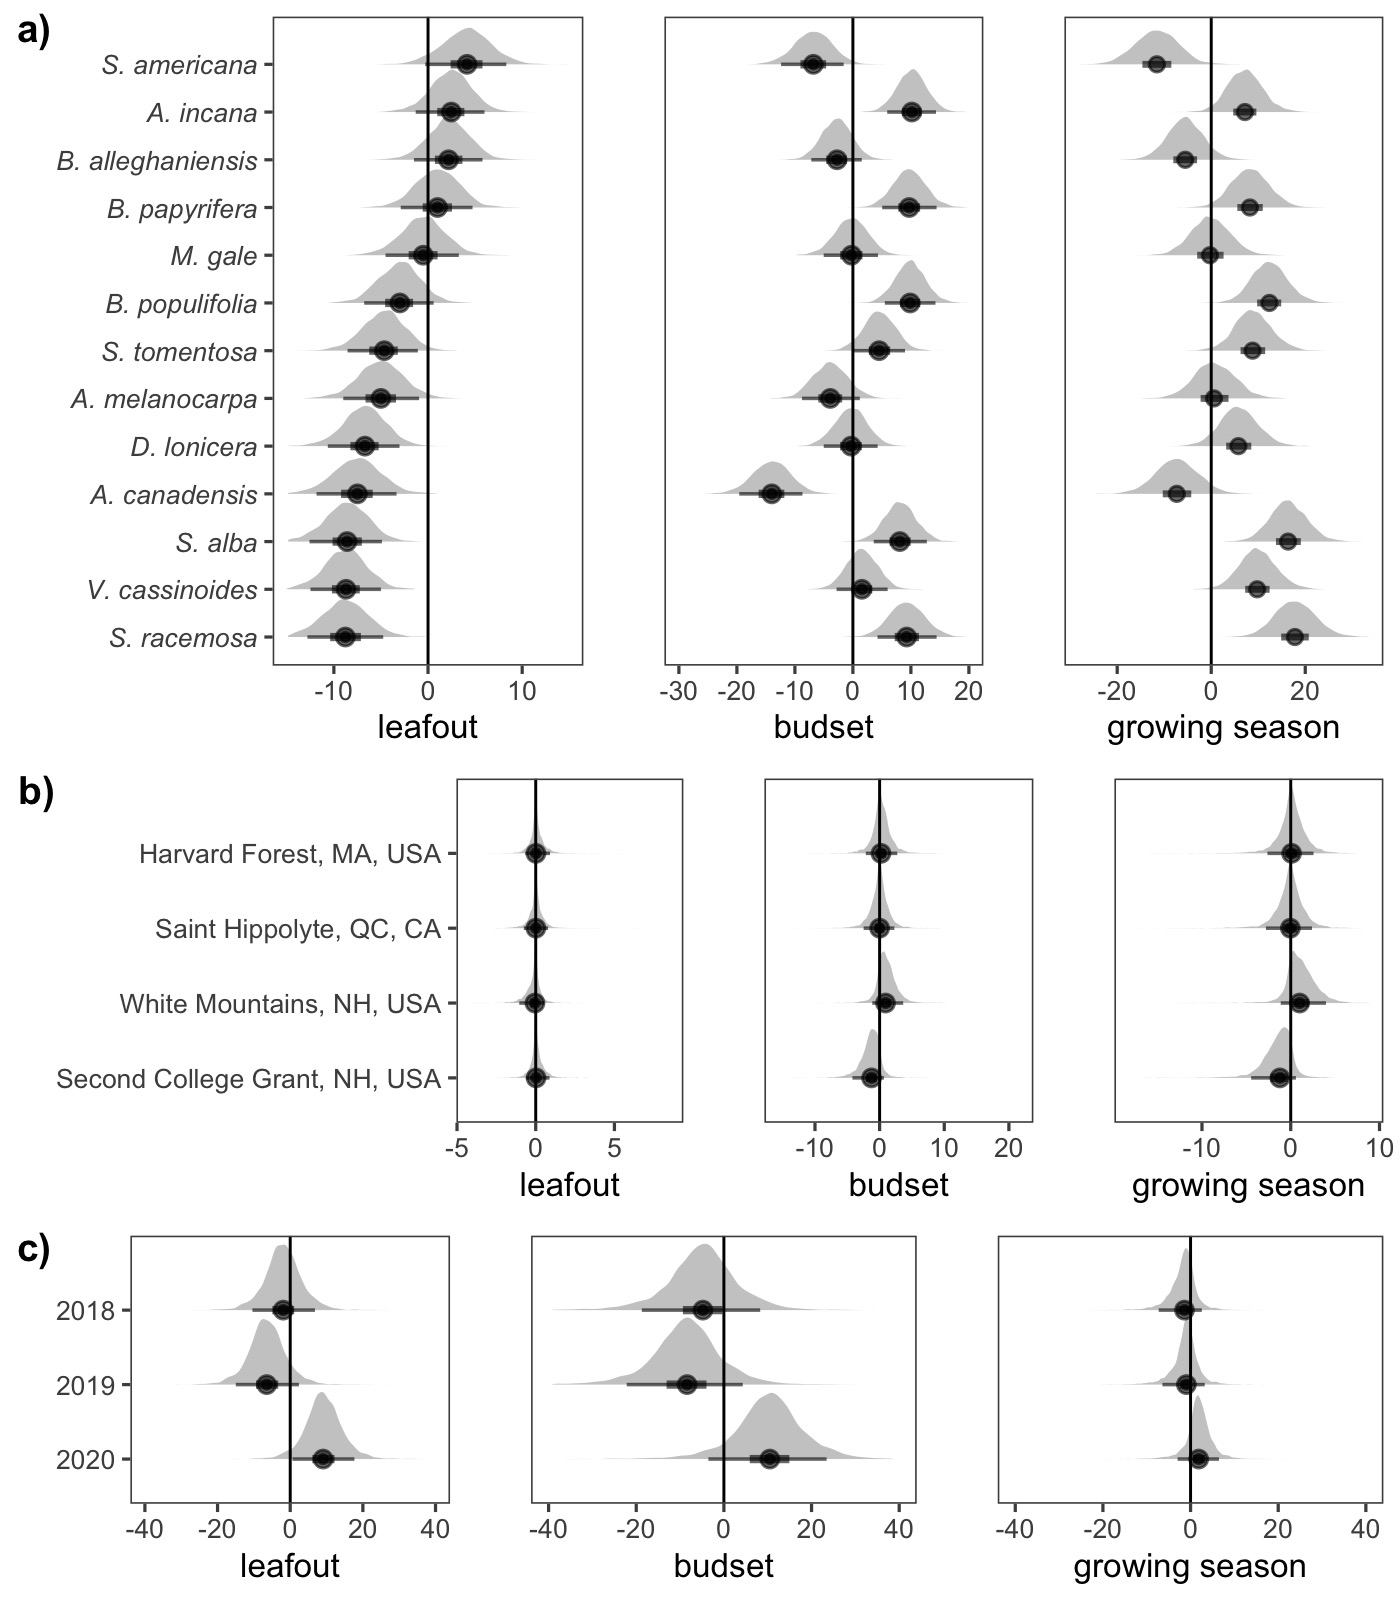
\includegraphics[width=.7\textwidth]{..//analyses/figures/var_parts.jpeg}
    \caption{Difference in leafout, budset and calendar growing season length partitioned between species (a) populations (b) and years (c). Point represent the median effect size estimate, and bars the 50\% uncertainty intervals. The grey distribution depict the full uncertainty estimate around the estimate.}
    \label{fig:vapar}
\end{figure}

%dl2024Sept20 such a cool result! 
%cjc2024Sept25 - agreed, this is awesome!
\begin{figure}[h!]
    \centering
 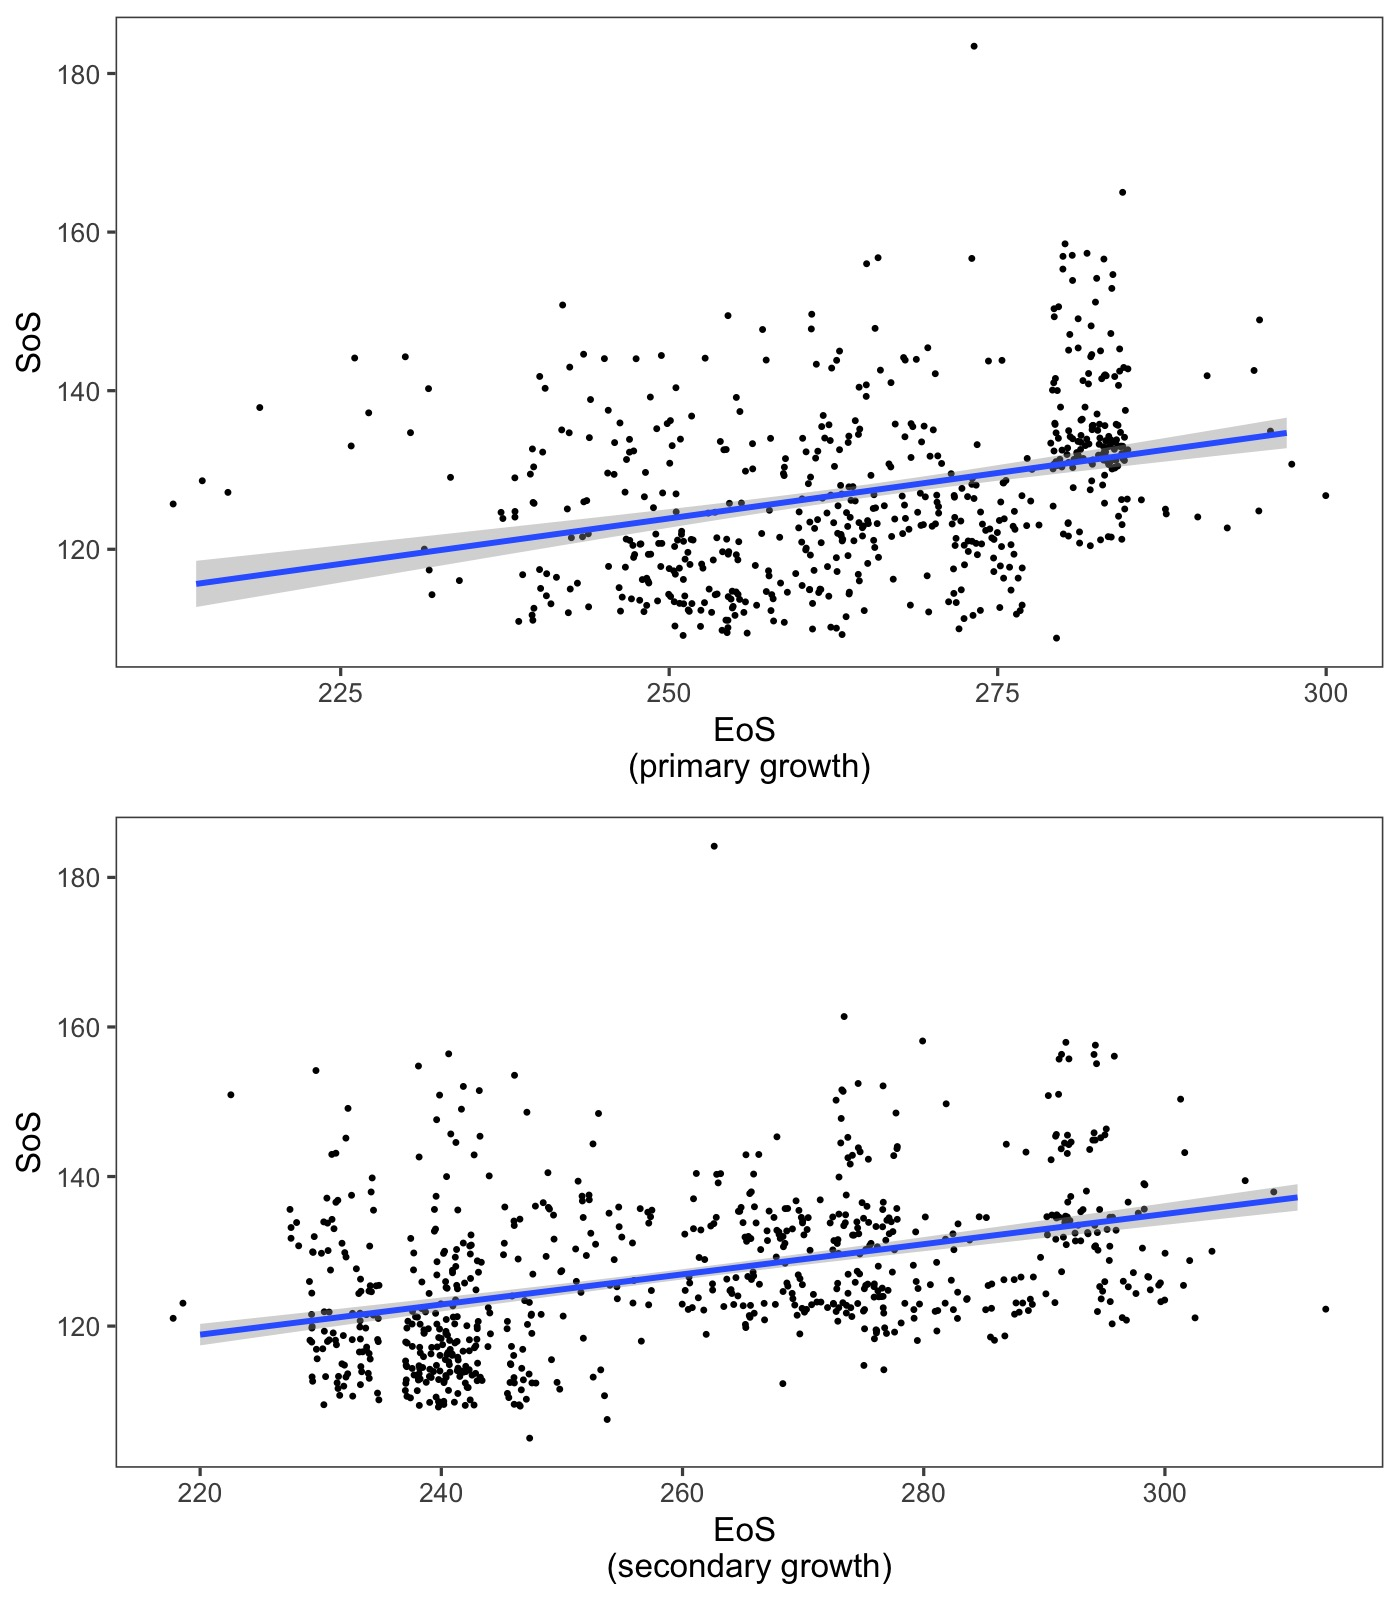
\includegraphics[width=.7\textwidth]{..//analyses/figures/primarygrowingseason_modplots.jpeg}
    \caption{The relationship between Start of Spring (SoS; calendar day of leafout) and growing season length differs between the calendar growing season and the thermal growing season. An increasing later SoS resulted in a shorter calendar growing season (panel a) and this pattern was consistent across species in our study (panel b). In contrast, an increasing later SoS resulted in a longer thermal growing season (panel c) though this effect was stronger for species that typically leafout earlier in the season---panels in c) are display in the typical order of leafout among species. The blue trend lines represent the mean effect of SoS timing on growing season length and black lines represent 1000 draws from the posterior distribution as a measure of uncertainty. Points in a), and c) represent the raw data. \textbf{to do: rename x-axis on b and d and write our the species names}}
    \label{fig:thermcal}
\end{figure}

%dl2024Sept20 can we add a legend defining the light and dark colors? I think the dark and light colors are switched in c.
%dl2024Sept20 I really like a, and what we are trying to show in b and c, but could see how the scale of the x-axis lessens the point we are trying to make.  Could we add some sort of transparent polygon in the background to show the thermal growing season and illustrate that the growth is outside of this window in b but not in c?
 \begin{figure}[h!]
    \centering
 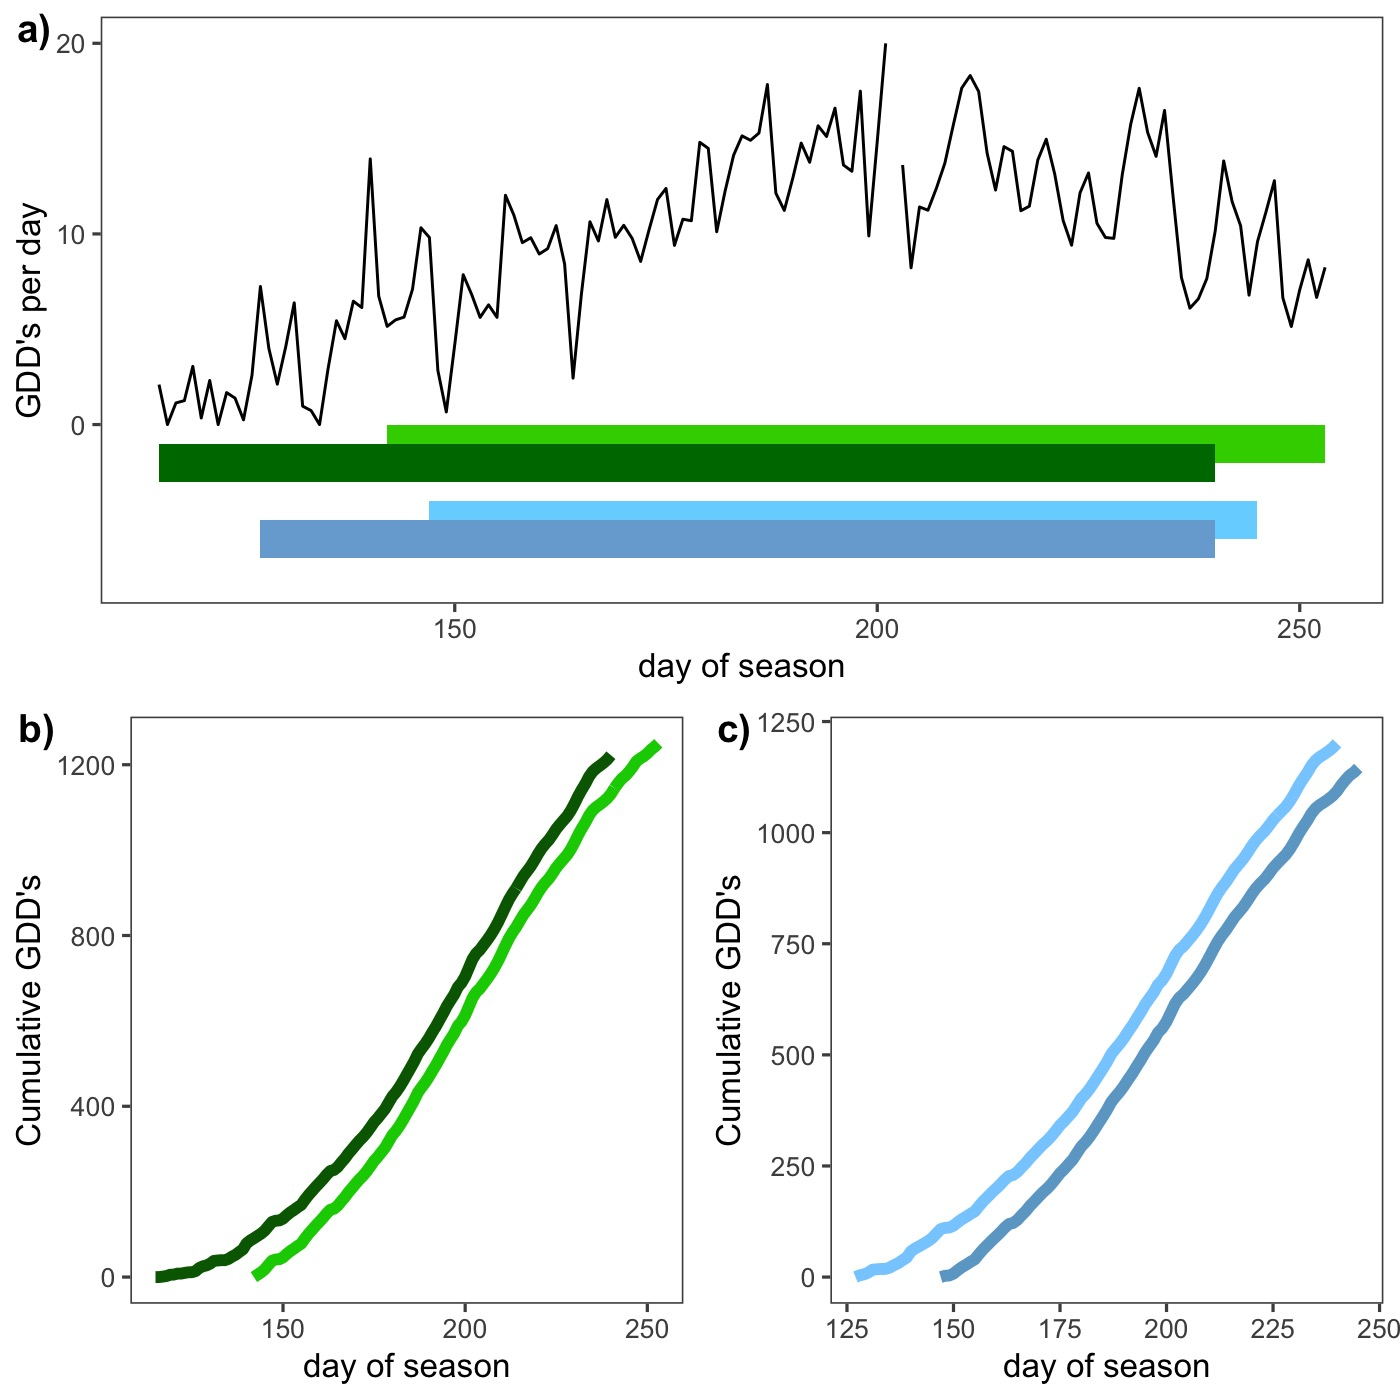
\includegraphics[width=.5\textwidth]{..//analyses/figures/aronia_examp.jpeg}
    \caption{Thermal conditions vary across the calendar growing season, which can generate a complex relationship between the calendar and thermal growing seasons. Panel a) depicts the daily heat sums at the Weld Hill Research Building in 2019 and the calendar growth season of early and late leafing individuals of \emph{Aronia melanocarpa} (green bars) and \emph{Myrica gale}(blue bars). Despite the fact the the early individual of \emph{A. melanocarpa} leafs out 24 days before it's later con-generic and only sets bud 13 days before it (i.e., it has a 14 day longer calendar growing season) it's thermal growing season is shorter (panel b) because most of its growth advantage (explain this better) takes place in the unfavorable early spring. In contrast for \emph{M. gale} where both the early and late individual leaf out later in the spring, the 20 day head start and 5 day earlier finish of the earlier individual (15 day longer calendar growing season) results in a longer thermal growing season for it as well (panel c)}.
    \label{fig:concept}
\end{figure}

\bibliography{..//refs/wildhell.bib}

% cjc2024Sept25: maybe we consider including sample sizes across the populations?
\begin{table}[ht]
\centering
\caption{Species list} 
\label{listSp}
\begin{tabular}{lr}
  \hline
Species & functional group \\ 
  \hline
  \emph{Acer pensylvanicum} & tree    \\ 
  \emph{Acer spicatum} & tree   \\ 
   \emph{Alnus incana} & shrub  \\ 
   \emph{Amelanchier canadensis} &  shrub  \\ 
  \emph{Aronia melanocarpa} & shrub \\ 
  \emph{Betula alleghaniensis} &  tree\\ 
  \emph{Betula papyrifera} &   tree\\ 
  \emph{Betula populifolia} &  tree \\ 
  \emph{Diervilla lonicera} &  shrub \\ 
  \emph{Myrica gale} &  shrub\\ 
  \emph{Sambucus racemosa} &  shrub\\ 
  \emph{Sorbus americana} &  shrub\\
  \emph{Spiraea alba} &  shrub \\ 
  \emph{Spiraea tomentosa} &   shrub\\ 
  \emph{Viburnum cassinoides} &  shrub \\ 
  \end{tabular}
\end{table}

\end{document}


